\chapterauthor{Author Name}{}

\chapter{Natural Language Processing}

In this chapter we introduce modern NLP libraries, techniques and their applications.
This chapter will focus on deep learning methods and less on computational linguistics that require nuanced knowledge of linguistics.
We explore what it means to represent words and sequences of words with rich numeric representations that are better-suited toward modern computational tasks.
We aim to capture some of these modern fine-tuned representations that are specially catered toward a semantic lexicon for medical language.
We use these representations and aforementioned tools to showcase a modern reference implementation leveraging PyTorch, PyTorch Lightning and the Huggingface Transformers library.
To wrap it all together, we walk through a complete example that highlights best practices that encourage reproducibility and allow for systematic iterative improvements.
\\

\noindent This includes:
\begin{itemize}
\item An introduction into fundamental NLP concepts
\item Bootstrapping techniques to iterate on a dataset in the low-resource setting
\item Storing of a reference dataset in a publicly-accessible location
\item Downloading, caching, loading, splitting, and preprocessing of the data
\item Setting up of a cloud-based GPU workstation (?) (--this might be overkill for now, but keep if we can)
\item VSCode (?)
\item Monitoring the training run:
  \subitem Logging and experiment tracking
  \subitem Learning curves
  \subitem Metrics
\item Hyperparameter tuning, some tricks of the trade
\item Offline evaluation and sanity checking
\end{itemize}
We will keep the discussion focused on tasks in epilepsy, using a running example of SUDEP prediction from electronic medical record (EMR) notes.
Many of the concepts introduced here are very general and are straightforward translations to domains outside of SUDEP prediction, epilepsy, and even NLP.

\section{Introduction to Natural Language Processing}

Natural language processing (NLP) is a field of computer science that deals with the extraction, processing, and understanding of human language.
It is known as the field of computer linguistics, and is a subfield of artificial intelligence.
Common NLP tasks include sentence segmentation, tokenization, part-of-speech tagging, named-entity recognition, parsing, question answering, summarization and classification.

How can we teach a computer to perform these tasks?
The first challenge is that computers, at their core, only understand numbers.
So first we need to think about how words can be represented with numbers such that we can perform calculations on them.
The numbers should allow the computer to assign meaning to words and their context with other words around it.

There is no perfect way to represent language in this numeric fashion. The best we can do is to capture representations that we feel capture the \textit{syntactic} features of text, as well as \textit{semantic} features of text.
Syntactic information refers to grammatical constructs and the way that words are put together in a language. Semantic information refers to the meaning of this body of text. Such distinctions are fundamental concepts in computer science
and date back to the very foundations of information theory. \cite{shannon48}. Much of this chapter, as well as much of the current work in the field of computational linguistics is centered around finding better and better representations that capture both types of this information.

How do we begin to choose these representations? Do we choose to represent words, or perhaps individual letters? Do we choose all the words? What do we do with punctuation and numbers?

\subsection{Vocabularies and Words}

In NLP, the set of unique words in a corpus is called a \textit{vocabulary}. While \textit{the} is the most common word in the English language, it is only one entry in a very large vocabulary table. A rare word like \textit{hemispherectomy} is also one
entry in this table. Both \textit{apple} and \textit{apples} might be separate entries in our vocabulary table. Generally the first step in many NLP systems is defining this vocabulary and the rules behind which words are in this table and which words are not.

The process of splitting text into separate smaller units, in this case words, is known as \textit{tokenization}. When we run many NLP tasks, we almost always preprocess our text by putting it into one of these tokenizers. The output tokens,
in this case words, are the indexes in our lookup table to different numeric representations that can be understood by a machine. There are a number of great tokenization libraries that are open source, and you should always use them rather than
try to implement this yourself.

\begin{python}
  # Example 1: Spacy Tokenization Using Medical Words

  import spacy
  sample = "After a temporal lobe resection, the atonic " \
           "and clonic seizure frequency fell by 50%."

  nlp = spacy.load("en_core_web_sm")
  english_vocab = set(nlp.vocab.strings)
  spacy_document = nlp(sample)

  for token in spacy_document:
      found = "found" if token.text in english_vocab else "NOT FOUND"
      print("{}: {}".format(token.text, found))
\end{python}

The discrete numeric entities created in Example 1 are the indexes for our representations. The tokenizer system did much of the magic under the hood, lowercasing and standardizing text and creating special tokens for punctuation and numbers.

When we build a vocabulary $V$, we define a preset vocabulary size $|V|$. There is a tradeoff in your choice of $|V|$. If you choose a number that is too small, then
your system will only recognize a few words and lose a lot of important task-specific vocaublary. However, if you include the entire english language, your system will be slow, expensive, and not perform as well.
Commonly this number is set around 20,000 - 40,000 words in English, though it can be much larger.

Often a vocabulary will include special tokens that make our lives easier when working with NLP tasks. Common special tokens include:
\begin{itemize}
  \item \pythoninline{[EOS]} - An end of sentence/input marker.
  \item \pythoninline{[PAD]} - Special inputs to ignore, usually following an EOS marker.
  \item \pythoninline{[SEP]} - A separator, which can be used in inputs that contain multiple sentences or samples.
  \item \pythoninline{[OOV]} - Out of vocabulary, also commonly represented as [UNK] (unknown), which is used when we come across a word that does not exist in our vocabulary.
\end{itemize}

The out-of-vocabulary token is of particular importance in medicine. If we load a vocabulary with 30,000 words, often these are roughly the most common 30,000 words in the English language. We will still have a few [OOV] tokens
for rare words. However, just because a general system chooses its vocabulary based on word frequency does not mean that this is the best choice of vocabulary for the task at hand. Medical corpora have a very different word frequency
distribution than non-medical corpora, particulary because of nuanced vocabulary that is absolutely crucial.

%TODO - add some epilepsy-themed example that throws away all the epilepsy words%

In Example 1 above, notice the importance of the words that have been thrown away. If this sentence were to be loaded into a machine as-is, we might be losing far too much information because we have to nearly all of the relevant terminology with OOV tokens.

We will address this issue in the ensuing sections. For now, suffice it to say that we should make sure our vocabularies are catered toward our task at hand or are built in such a way that they can still extract signal from these tokens.

\subsection{Word Representations}

Given that we have defined a vocabulary $V$ of words, these are the keys to our lookup table of numeric representations. But what do we store in that table as the value?

A simple way to achieve this representation for $V$ is to assign each word a unique integer $i$.
The word is then represented as a vector $w$ of length $|V|$ with all zeros and a one at index $i$\footnote{This is also known as a one-hot encoding}.

\begin{python}
  have = [1, 0, 0, 0, 0, 0, ... 0]
  a    = [0, 1, 0, 0, 0, 0, ... 0]
  good = [0, 0, 1, 0, 0, 0, ... 0]
  day  = [0, 0, 0, 1, 0, 0, ... 0]
  ...
\end{python}

We could now represent a sentence as the sum of the word vectors $S = \sum_j w_j$. This representation is suitable as input for any classification algorithm (such as logistic regression or a decision tree), to make a prediction about our target variable, e.g. whether the sentence is relevant to our epilepsy task.
This simple representation fulfills our requirements but comes with some drawbacks:
\begin{itemize}
    \item We implicitly assume that each word in the sentence is equally important.
    \item Each word is equally similar to every other word (e.g. by taking the euclidian distance between word vectors).
    \item The representation is invariant to reordering of the words.
\end{itemize}
The first point is a problem, because as we add more word vectors together, the sentence reperesentation will converge to the global average and drown out any signal relevant to the specific sentence at hand.
To address this we can instead write a weighted sum $S = \sum_j \lambda_j w_j$, where each word vector is weighted by its importance $\lambda_j$, and there are statistical methods we can use to compute an importance value\footnote{TF-IDF}.
For example a word like \textit{the} is very common and appears in many different contexts.
It is unlikely that there is a lot of signal we can extract from it.
On the other hand, a word like \textit{epilepsy} will be much more rare and specific to a given task, and we would like to raise its importance.
This has the net effect of allowing us to find a good representation for larger word sequences.

To address the second point, we will be touching on a very important concept, not just relevant in NLP, but also in the world of ML in general: Embeddings.

\subsection{Embeddings}
\label{embeddings}
An embedding is a representation of a vector space that captures the similarity between the entities we are encoding, where entities can be words, images, e-commerce products, movies, houses, and many other data modalities.
Scientific progress in the field of ML is often directly about finding algorithms that can learn high-quality robust embeddings in an efficient and scalable way, and the final performance of a given architecture is largely determined by the quality of the embeddings it learns.

To illustrate this concept, we will be talking briefly about one of the earliest algorithms that has been used to learn embeddings for words: \textit{word2vec} \cite{mikolov13}, a technique pioneered by a team led by Thomas Mikolov.
The idea behind \textit{word2vec} is to set a word into context with the words surrounding it. In NLP, the study of techniques that determine the probability of a given sequence of words is known as language modeling.

For example the word \textit{epilepsy} may appear in the context of words like \textit{symptom}, \textit{medication}, or \textit{episode} and vice versa.
However, we would not expect that \textit{epilepsy} would appear in the context of words like \textit{volleyball}.

We then translate this idea into a training task:
Given the sum of the one-hot encoded word vectors of the words surrounding the target word, map it to the one-hot encoded vector of the target word.

This is a task that can be solved by a neural network with the following setup:
Add a layer $l_1$ that maps from the input dimension (of size $|V|$) to an intermediate dimension of size $h$ and then another layer $l_2$ that maps from the intermediate dimension to the output dimension (of size $|V|$).
Here $h$ is what is called embedding dimension and $h << |V|$.
\begin{figure}
  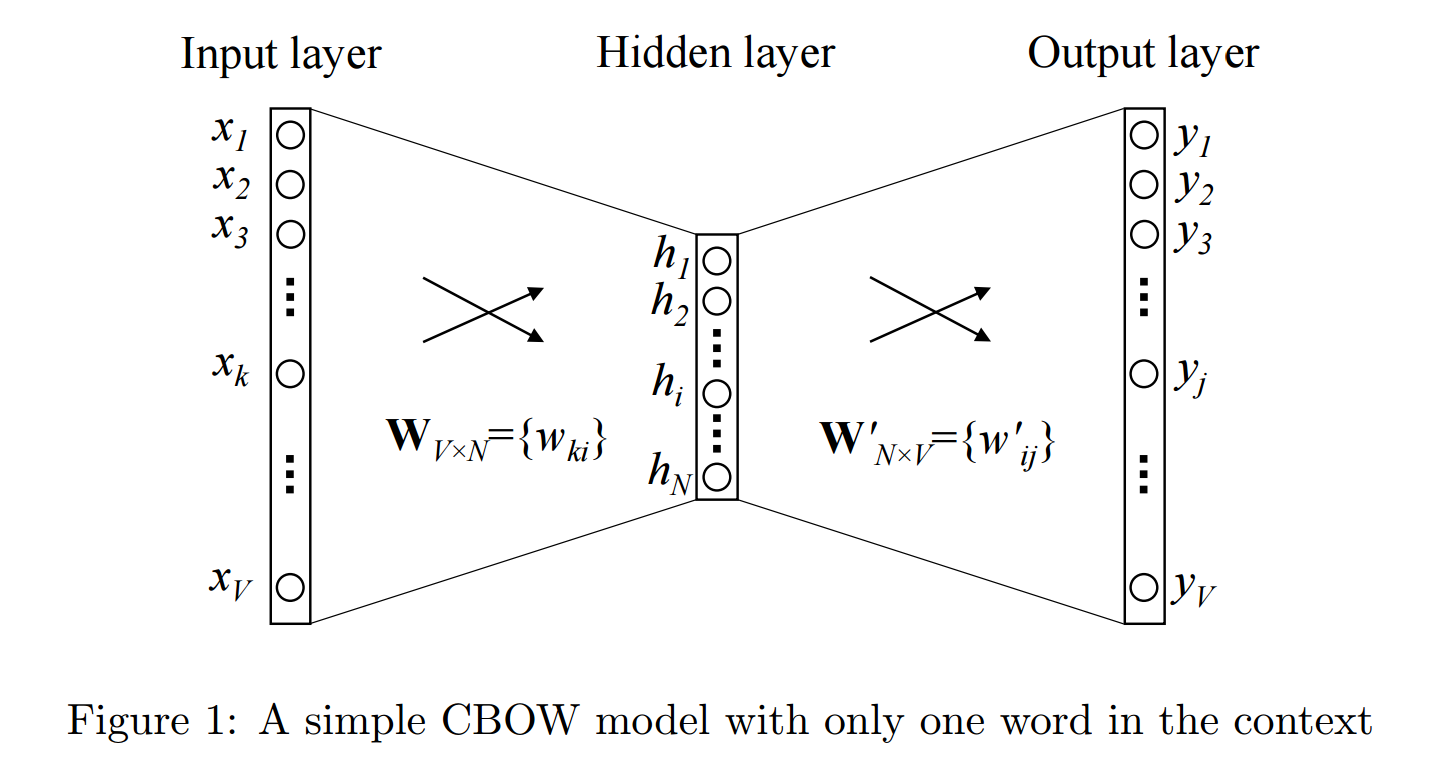
\includegraphics[width=\linewidth]{chapters/NLP/figures/word2vec.png}
  \caption{Word2vec}
  \label{fig:word2vec}
\end{figure}
While $h$ is generally a hyperparameter that can be optimized at a later stage, a reasonable choice is to use a value according to the rule of thumb:
\begin{equation}
  h \approx 4\sqrt[\leftroot{3} \uproot{3} 4]{|V|}
\end{equation}
For a vocabulary size $|V| = 30000$ this comes to a value of about $50$.
During training, the network will learn to encode the original sparse indicator vectors in a way that preserves the maximum amount of information necessary to predict the target word, while being forced to squeeze the information through the low dimensional bottleneck.
An interesting side effect of this approach is that we can use part of the network to encode a given word in $V$ by using for example the inverse of $l_2$ as a lookup table.
The vectors that we obtain from this lookup table are called word embeddings and they have some very useful properties:
\begin{itemize}
    \item Similar words tend to be close together (e.g. in terms of euclidian distance).
    \item Averaging word embeddings of a sentence will give us a more robust representation than our naive approach.
    \item We can perform some arithmetic, such as adding and subtracting the embedding vectors to traverse the space.
\end{itemize}
\begin{figure}
  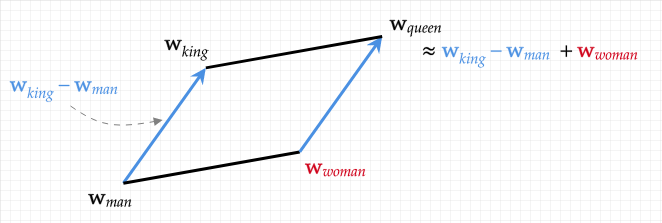
\includegraphics[width=\linewidth]{chapters/NLP/figures/king-man+woman.png}
  \caption{Word2vec}
  \label{fig:kingmanwoman}
\end{figure}
These properties also imply that the representions for two sentences will be close together if they are semantically similar, which will make the job of, say, a downstream classifier much more straightforward - it only has to slice the embedding space.
The hard part of understanding the meaning of the sentence is already done.
Since the training data can be generated from just raw text, it is sufficient to train the embeddings once on a very large corpus\footnote{GloVe} and then reuse them, in effect giving us a headstart when building task-specific models.
Instead of also having to learn what words mean, and some of the syntactic rules behind written language, we can get a head start on this and focus our computational resources on adapting this knowledge to a specific task.

This underlying assumption that similar neighboring words share a semantic similarity to center words is powerful, and at the heart of many modern training objectives for embeddings that are used in many downstream ML systems.
We do not inherently inject a great deal of model bias, but rather rely on having a large enough training set that the word vectors will become meaningful representations with respect to one another.
A corpus such as Common Crawl\footnote{Common Crawl Link}, which contains roughly 840 billion tokens of over two million unique words, provide such scale.
There are other corpora used in these unsupervised processes, one such common candidate being a collection of all Wikipedia articles.

In practice, one training objective can be to use the distributed representation of a set of context words to guess a center word. This is known as the continuous bag of words (CBOW) model.

Consider a training document describing patients with epilepsy, where we are attempting to train a model with a predefined vocabulary $V$ of the top For a vocabulary $V$, where we have chosen the top $|V|$ most common words in English to learn.
The document being chosen in this training iteration may contain the following excerpt:

\begin{verbatim}
  ... recommended administering Lamictal to treat their
  focal seizures, the patient continued experiencing
  symptoms though reported a 50% reduction in ...
  \end{verbatim}

In training our word embeddings, we will randomly mask one of the words, in this case \textit{patient}.
Our model makes use of an additional parameter, a context window size $c$, that helps to provide necessary context.
If we choose $c = 8$, our training sample would become

\begin{verbatim}
  ... lamictal to treat their focal seizures, the [MASK]
  continued experiencing symptoms though reported a 50 % ...
  \end{verbatim}

For a given center word at index $i$, we consider previous words at indexes $i-1$, $i-2$, ..., $i-c$, and all subsequent words at indexes $i+1$, $i+2$, ..., $i+c$.
In our word sequence $S$, we may then choose to sum the word vectors of each of these context words.
Our context input can be written as:
\begin{equation}
  \sum_{ \substack {j=-c \\ j \neq 0}}^c w_{i+j}
\end{equation}

Our task is then to predict a probability distribution over the size of our vocabulary $|V|$, where the target is a vector of all 0's with a 1 at the index in the vocabulary for the word \textit{patient}.

There are a few additional takeaways from this example.
Note that we will address many of these in the sections to follow.
\begin{itemize}
  \item The training process will likely consider this text many times, and mask out different words in each iteration.
  \item Our processed sentence is slightly modified from our original input.
  Notice that the number and percent symbol are split, and that Lamictal is lowercased.
  \item The word \textit{patient} can also be an adjective.
  Our \textit{patient} embedding will also capture this meaning in our model, dependent upon how often it is used with that meaning.
  \item If our context window is too small, we lose information.
  If it is too large, our signal becomes fuzzy as we converge to the global mean vector.
\end{itemize}

What if we choose to use only a center word, and have our model predict all of the surrounding context words?
This is a common training technique for embeddings as well, and is known as the Skip-Gram model.

\subsubsection{Spacy Example}
This is placeholder text

\subsubsection{Character and Subword Embeddings}

In Example 1, we covered the issue of missing vocabulary that is frequently encountered when using word-level tokenization.
However, there are other strategies that are commonly used that help to avoid this issue.
One such simple way around out-of-vocabulary tokens is to use character-level tokenization.
Instead of having a vocabulary that is tens of thousands of words long, you only have a vocabulary that contains the characters in
your language, with the addition of punctuation, digits, and a few special tokens for sentence and word marking.
As long as tokenizer is able to mark which characters start a word and which characters are continuations of a word, then the original sequence of words can always be recovered.

Unfortunately, the tradeoff for a small vocabulary size with no unknown word entries is that the length of tokens to represent a sentence is clearly much larger.
Empirically, these models do not perform as well, partially because of this sequence but also because of the loss of information that is represented in word vectors.

In practice, the best models are often somewhere in the middle, in what is known as word-piece, or subword, vocabularies.
These tokenizers and vocabularies contain a rich set of common words, but also have subword units that can be used to piece together out-of-vocabulary words.
These subword units behave like normal word vectors and can store semantic and syntactic information.


\begin{python}
  # Example 2 - Wordpiece Tokenizers

  from transformers import BertTokenizer

  sample = "After a temporal lobe resection, the atonic " \
           "and clonic seizure frequency fell by 50%."

  bert_tokenizer = BertTokenizer.from_pretrained('bert-base-uncased')

  encoded_ids= bert_tokenizer.encode(sample)
  encoded_tokens = bert_tokenizer.convert_ids_to_tokens(encoded_ids)

  for token, id  in zip(encoded_tokens, encoded_ids):
    print("{}: {}".format(token,id))
\end{python}

In example two,

% \subsubsection{Vocabularies and Medical Embeddings}
% This is placeholder text.
% Would \texttt{BioBERT} and \texttt{Bio\textunderscore ClinicalBERT} here be worth mentioning?
% If not, should maybe follow the transformers section

\subsection{Transformers}
There have been significant advancements in ML due to a variety of factors, such as the availability of larger and larger datasets, as well as ever increasing computational power at lower and lower prices, better software tools, libraries and model architectures.
Especially the advent of deep learning (DL), fueled by the emergence of GPUs from about 2012, enabled scaling to many orders of magnitude larger datasets and models.
The common wisdom before DL was that as the number of parameters in a model increases beyond a certain threshold, it tends to overfit the training data, leading to poor generalization when deployed in the real world.
Deep Learning based models empirically do not seem to exhibit this behavior, and instead tend gain performance as they get bigger, albeit more slowly.

Until recently, building strong NLP systems required deep understanding of language and its structure, as well as large amounts of data, even when relying on pre-trained word embeddings - the resulting systems were often still brittle.

In recent years some surprisingly powerful architectures and pre-training regimes have emerged that build on the concepts we have discussed here, most notably under the name of \textit{Transformers\footnote{BERT, GPT}}, that address the last bullet point of our representation's shortcomings.

The details of the inner workings are beyond the scope of this tutorial, for now it suffices to know that they are able to learn robust sentence embeddings with a fine grained understanding of syntactic structure, semantics, and general knowledge of the world.
In fact, they can be considered near the level of a human that just knows the English language (or other languages), along with a broad array of factual knowledge about the world (think Wikipedia).
Just like a human, they can be taught specialty knowledge that is relevant to a given task, in ML we would say we \textit{finetune} them.
% Where these models to date generally fall short is in terms of logical inference.
This paradigm shift has led to a step function improvement in terms of performance and sample efficiency in a wide variety of NLP tasks where Transformers are the defacto state of the art.

In the following sections, we will discuss a broad set of problem statements Transformers are suitable for, along with a set of techniques a practitioner can employ to arrive at robust solutions, even with limited data.

\subsubsection{Pre-training}
Modern DL based systems, such as the aforementioned Transformer architectures, are pre-trained on gigantic datasets\footnote{BooksCorpus (800M words, Wikipedia 2,500M words)}\cite{bertpaper} and can be downloaded for free\footnote{Huggingface}.
Starting with a model pre-trained on a broad set of topics significantly reduces the amount of task specific training data required to achieve a given performance.
Furthermore, it may be helpful to start with a model that is pre-trained on more domain specific datasets such as \texttt{BioBERT\cite{DBLP:journals/corr/abs-1901-08746}} or \texttt{Bio\textunderscore ClinicalBERT\cite{clinicalbert}}, or pre-train your model from scratch.

\section{NLP Tasks in Epilepsy}

% This is a placeholder title.
% A couple pages here might do nicely as example studies for some important techniques for epileptologists.
Now that we have an understanding of some of the basics of computational representations of language data, let us take a look at some of the modern use cases for NLP in industry, catered toward epileptologists and other medical practitioners.


\subsection{Unstructured Text - Retrospective Research}
Within the medical field, there are many sources of unstructured text that are primarily aimed as a either a communication channel between specialists, or a way for patients to pass information that isn't captured in a structured format.
Clinical Notes, Progress Notes, Operative Notes, Discharge Summaries, Pathology Reports, Surgery Reports; all of these sources carry information, but traditionally require experts in the field to extract it.
If we can teach systems to read through this unstructured text and perform respectably close to these experts, we can perform large-scale clinical retrospective research much faster and at a much lower cost.

Example:
https://academic.oup.com/jamia/advance-article/doi/10.1093/jamia/ocac018/6534112

\subsection{Unstructured Text - Quality of Life}
This is a placeholder for some of the work that is done on the Quality of Life surveys for the INJS Seizure Tracker datasets.

\subsection{Text Preprocessing and Tokenization}

Placeholder.

\subsection{Named Entity Recognition and PII}

This is a working title. NER is an important problem in medicine, for PII if nothing else, and I figure we could go through some basics of using it with Spacy, NLTK, or Stanford NLP here.

The reluctance towards data sharing and common formats in the medical domain has hampered progress significantly.

Stopwords would be worth mentioning?

\subsection{Mining Unstructured Text and Clinical Documentation}



This is placeholder text. Talk about clinical documentation and EHR notes, and other forms of unstructred text, being used for downstream classification tasks.
Then, give some examples of them, and what these people did, and possibly how transformers could probably improve this work greatly.

\subsection{Clinical Trial Matching and Eligibility Prescreening}

This is a placeholder text. https://www.nature.com/articles/d41586-019-02871-3

\subsection{Surgical Candidacy}

This is placeholder text

\subsection{Avoiding Epilepsy Misdiagnosis}

This is placeholder text. https://www.ncbi.nlm.nih.gov/pmc/articles/PMC4419916/

\section{Research Process}
Part of any research process is rigorous record keeping to ensure experiments can be independently and reliably reproduced.
While researchers keep meticulous journals, when dealing with software this bookkeeping can be largely automated.


\subsection{Version Control}
Software engineering primarily relies on version control systems, such as GitHub, to keep track of code changes.

....

\subsection{Experiment Tracking}
\begin{figure}[h]
    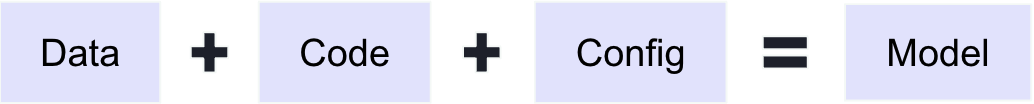
\includegraphics[width=\linewidth]{chapters/NLP/figures/model.png}
    \label{fig:model}
\end{figure}
An experiment is defined by the training code, data, and a configuration file.
When ML and Data Science are involved, the data generating process has to be documented.
In software engineering we say that code doesn't exist until it is "checked into" version control.
Similarly, data doesn't exist until it is stored in the cloud.
In addition to the raw data, we should also store documentation about how it was obtained, by whom, when, and if there have been any additional processing steps.
This should be done in a way that is easy to replicate and understand -- ideally it is documented in code as well.

While version control system are specialized to keep track changes in plain text files, they are not well suited for tracking changes in larger file objects.
To keep track of data (and model) versions the ML community has developed specialized tools\footnote{Weights\&Biases, Neptune}, which we have integrated into Sheepy.
As part of the training run a new experiment is initialized and all hyperparameters are tracked, along with the versions of all dependencies

In addition, these tools allow visualization of metrics, plots, comparison to previous experiments, as well as enables collaboration and sharing of results by directly linking to the tracked experiments.
While being able to repeat previous experiments is important, it is even better if we don't have to -- ML experiments can be expensive.
In addition it is useful to generate formally track \textit{artifacts}, where an artifact refers to a file that is not a code file, but is an important piece of data that is used to generate the results or is the result of an experiment, such as datasets and models.
The file itself is uploaded to a cloud storage service\footnote{Amazon S3, Google Cloud Storage}, and we store a reference to the file as part of the experiment.
Additionally we can store metadata, such as how many samples the data contains, the size and type of fields, when it was created etc..
This facilitates discovery, analysis, iteration, and collaboration.


\subsection{Data Preparation}
One should ensure that all steps necessary to obtain and pre-process the data are documented, ideally in code.
To this end, we provide utilities to handle
\begin{itemize}
    \item Data download
    \item Pre-processing
    \item Splitting into training, validation, and test sets
    \item Feeding data to the model during training
\end{itemize}

We'll go over each of these steps in more detail in the next sections.
The goal is to rerun an experiment from scratch with a single command and we build on top of PyTorch Lightning's \pythoninline{DataModule} class to handle these steps.
\subsubsection{Data Download}
Downloading the dataset from cloud storage and caching are handled in the \pythoninline{prepare_data} method and only executed once per run.
We will first check if the data is already cached, and if not, download it.

\subsubsection{Data Preprocessing}
In general, pre-processing refers to transformation steps we want to apply to the raw data to make it suitable to input into the model.
In NLP, raw text needs to be translated into arrays of integers that the model can map to embedding vectors (see Section \ref{vocabularies_and_words}) (Fig. \ref{fig:tokenization}).
\begin{figure}
    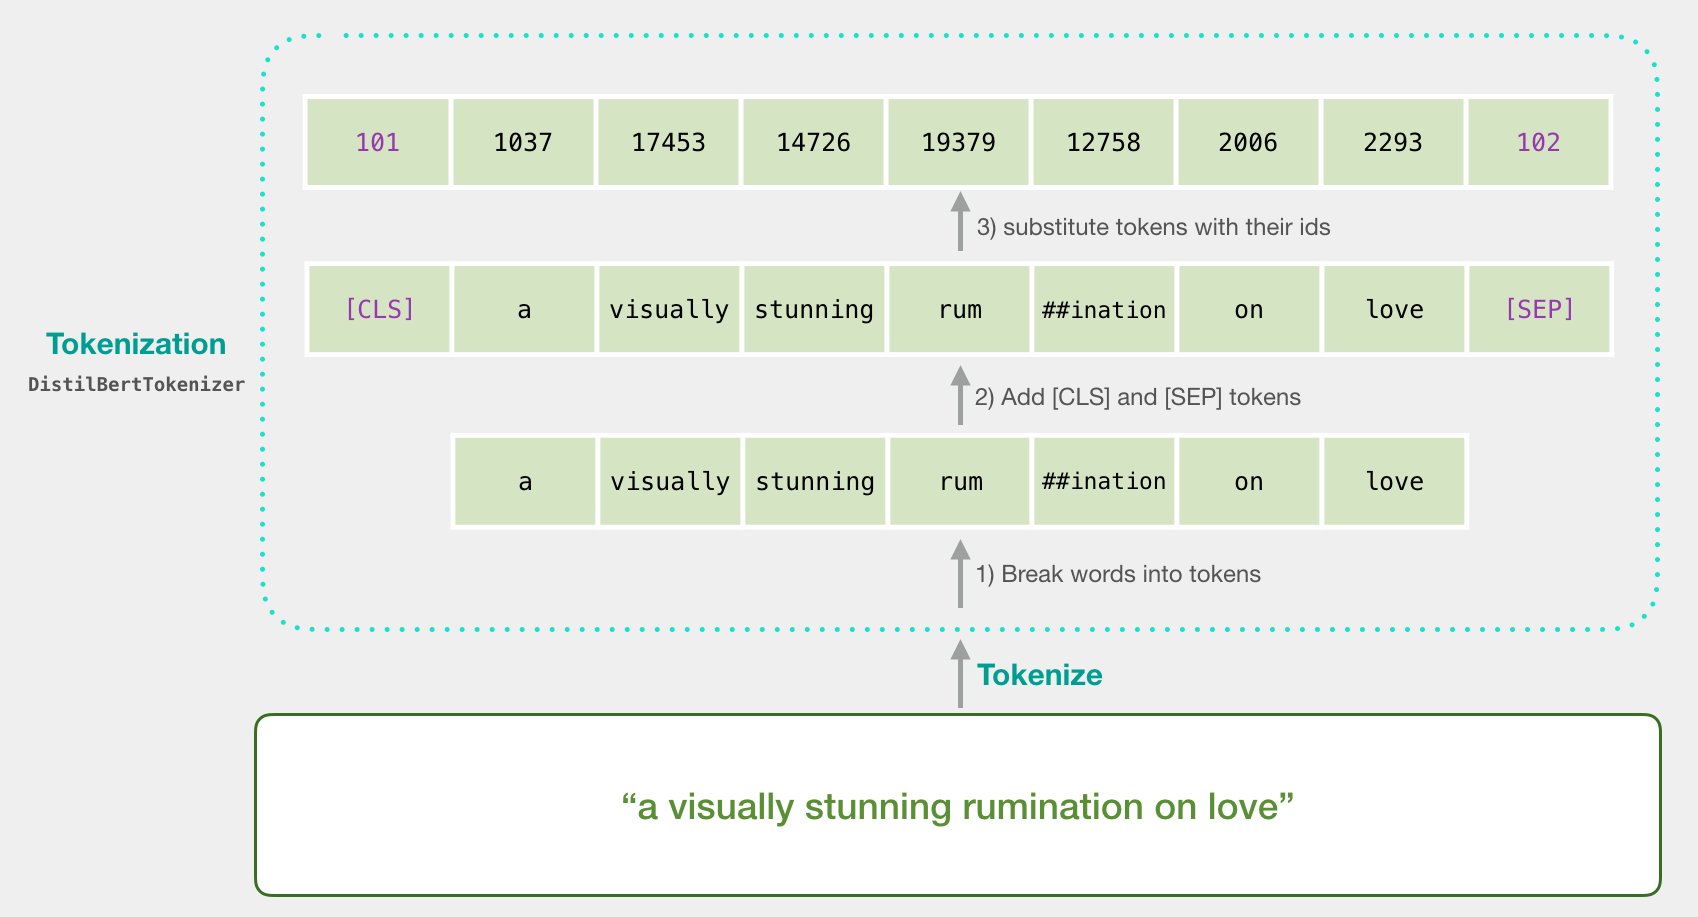
\includegraphics[width=\linewidth]{chapters/NLP/figures/tokenization.png}
    \caption{Tokenization}
    \label{fig:tokenization}
\end{figure}
These steps can be slow and in principle we need to do them only once per sample and cache the results.

\subsubsection{Data Splitting}
\begin{figure}[h]
    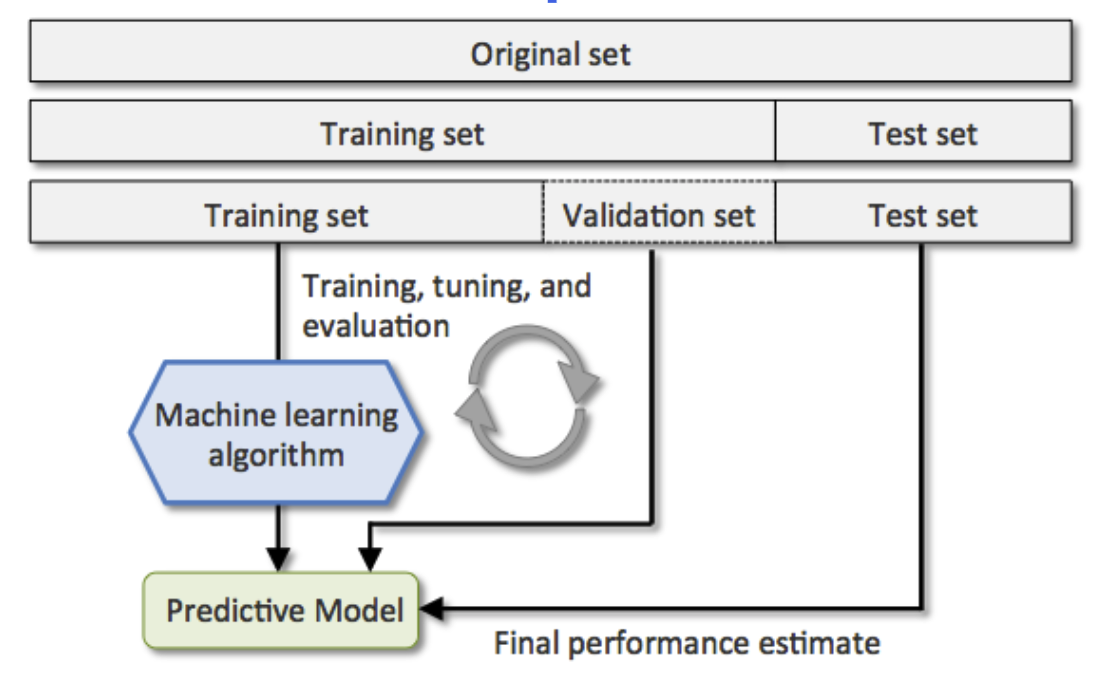
\includegraphics[width=\linewidth]{chapters/NLP/figures/data_splitting.png}
    \caption{Data Splitting}
    \label{fig:data_splitting}
\end{figure}
In order to evaluate the generalization performance of a model it must be tested on data it hasn't seen during training.
The dataset is therefore split into training and validation sets, typically at random (Fig. \ref{fig:data_splitting}).
It should be ensured the randomness is deterministic to reproduce results exactly, which can be achieved by setting a "seed" for the random number generator.
The validation set is used during training to monitor progress and tune hyperparameters.
In addition, it is good practice to hold out another portion of the data, the test set, which is never used during training, but only to report final results.
We otherwise run the risk of tuning hyperparameters to the validation data, thereby overestimating real performance.
Cross validation?
\subsubsection{Feeding Data to the Model}
\begin{figure}[h]
    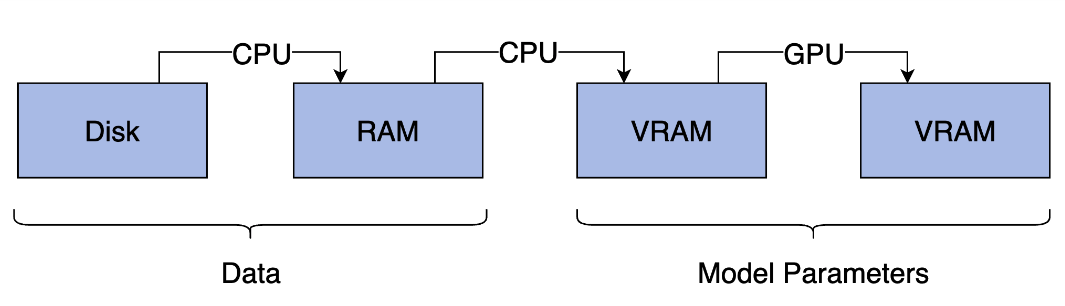
\includegraphics[width=\linewidth]{chapters/NLP/figures/ram_cpu_vram.png}
    \caption{Data needs to be moved from disk to RAM to VRAM so that it can be used to update the model parameters.}
    \label{fig:ram_cpu_vram}
\end{figure}
Model parameters are stored in GPU memory (known as VRAM); in order to update them, the GPU needs to process data from the training set.
After downloading the data from cloud storage it resides on local disk, from where it needs to be moved to RAM and finally VRAM.
Loading data into the model needs to be fast, or we run the risk of starving the GPU, meaning the GPU processes each batch of data faster than the CPU can deliver the next one, leading to low resource utilization and slow training.
We use PyTorch's \pythoninline{DataLoader} class to parallelize this process across multiple CPU workers.
A \pythoninline{DataLoader} is a wrapper around a \pythoninline{Dataset} which provides a stream of batches of data.
The \textit{batch size} is an important parameter that needs to be tuned on a case by case basis, as we will explain in the next section.

\subsection{Training}
\begin{figure}[h]
    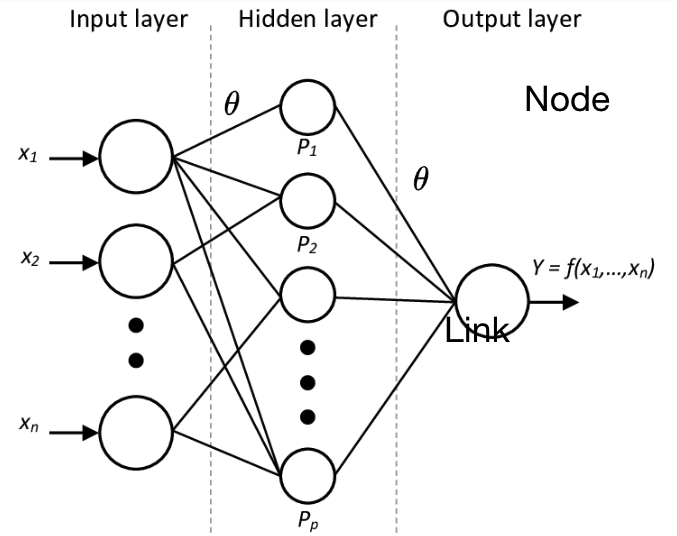
\includegraphics[width=\linewidth]{chapters/NLP/figures/model_architecture.png}
    \caption{Deep neural network architecture}
    \label{fig:model_architecture}
\end{figure}

While glossing over some details, model training can summarized in the following steps:
\begin{itemize}
    \item Given data pairs $(x_i, y_i)$, where $x_i$ is an input sample, and $y_i$ is the desired output
    \item Determine a function $f$, such that $f(\theta, x_i) \approx y_i$, where $\theta$ are model parameters and $f$ is the model architecture
    \item Define a loss function $L(\theta) = \sum_i L(\theta, x_i, y_i)$ that measures how close the model's output is to the desired output
    \item Optimize $\theta$ to minimize $L(\theta)$
\end{itemize}
\begin{figure}[h]
    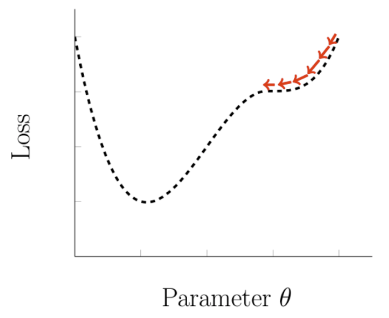
\includegraphics[width=\linewidth]{chapters/NLP/figures/loss.png}
    \caption{Minimizing the loss function}
    \label{fig:loss}
\end{figure}
Here the loss function can take on many forms, depending on the training task, we summarize some of the most common ones in table \ref{table:losses}.
\begin{table}
    \centering
    \renewcommand{\arraystretch}{1.3}
    \begin{tabular}{|c| c| c|}
    name & function & use \\[0.5ex] \hline
    Mean Squared Error & $\begin{array} {lcl} \frac{1}{N} \sum_{i=1}^N|\hat{y}_i - y_i|^2\end{array}$  & regression \\ [0.5ex]
    Binary Cross Entropy& $\begin{array} {r@{}l@{}} -\frac{1}{N} \sum_{i=1}^N (y_i \cdot log(\hat{y}_i) + (1 - y_i) \cdot log(1-\hat{y}_i)) \end{array}$ & classification \\ [0.5ex]
    \end{tabular}
    \caption{Loss functions}
    \label{table:losses}
\end{table}
Parameters in the last layer are then optimized according to the rule
\begin{equation}
    \theta \rightarrow \theta - \alpha \frac{\partial L}{\partial \theta}
\end{equation}
where $\alpha$ is called the \textit{learning rate} and determines the step size, the partial derivative of the loss function with respect to the parameters is called the \textit{gradient}.
For other parameters the rule is similar, but involves the application of the chain rule from calculus.
In modern architectures there are millions to hundreds of billions of parameters, and updating them efficiently is crucial.

\subsection{Metrics and Sanity Checking}
\label{metrics_and_sanity_checking}
Here we discuss metrics used to evaluate the performance of classification models.
While
We automatically generate metrics and plots relevant for text classification projects.

\section{Full Walkthrough - SUDEP Detection}

This is placeholder text

\section{Full Walkthrough - Brain Surgery and Financial Impact of Epilepsy}

In this section we will demonstrate how the techniques discussed above can be applied to a practical example within the field of Epilepsy.
Modern NLP techniques are a powerful tool to analyze large amounts of unstructred or semi structured text data, and we can employ them to develop a coding scheme and significantly reduce the time required to apply it to new data.

We are providing self contained code examples in the acompanying GitHub repository\footnote{https://github.com/chris-boson/epilepsy} that makes use of a general purpose NLP library\footnote{https://github.com/robmsylvester/sheepy} we have developed to make current industry standard tools and libraries more accessible to researchers and practitioners.


\subsection{Data Analysis}
For this section we started out with fairly small dataset ($\sim150$ rows) derived from survey responses regarding  impact and treatment of epilepsy\footnote{Seizure Tracker}:
\begin{displayquote}
    Do you have any comments on the financial impact of epilepsy?

    Do you have any comments about brain surgery in general?
\end{displayquote}
This dataset is small enough to manually inspect, but we the techniques discussed here scale well beyond.
\subsubsection{Embeddings}

\subsubsection{Dimensionality Reduction and Clustering}
\subsubsection{Cluster Labeling}
\subsubsection{Annotation}
We can use the cluster labels as a starting point to decide on a coding scheme. For the general comments we decided on the following labels:
\begin{itemize}
    \item Not eligible
    \item Last resort
    \item Would never do it
    \item Considering it
    \item Was Unsuccessful
    \item Was partially successful
    \item Was successful
    \item Side effects
    \item Risk
    \item Too expensive
    \item Complications
    \item Unknown outcome
    \item Unnecessary
    \item Cannot find origin
\end{itemize}

% - Large scale data analysis
%   - Embeddings
%   - Dimensionality reduction and clustering
%   - Cluster labeling
%   - Annotation
% - Research process
%   - Sheepy
%   - Reproducible results
%     - Experiment tracking
%     - Parameter tuning
%   - Metrics and sanity checking
%     - SHAP
%     - Analyze mistakes
%     - Inference

  % walk through the full process of developing a model to predict the financial impact of epilepsy, and how to do this in a way that is both accurate and scalable.

